%
% $Id: ch03_thework.tex
%
%   *******************************************************************
%   * SEE THE MAIN FILE "AllegThesis.tex" FOR MORE INFORMATION.       *
%   *******************************************************************
%
\chapter{Method of Approach} \label{ch:method}
This chapter is meant to explain the experimentation and testing process. It will discuss many of the decisions for what would be tested and how. It will also explain the qualifications that were necessary for a system to be experimented on.

\section{Test Environment}
% Algorithm \ref{widgmin} (from \cite{Fiori:2013}) shows a high-level description of an
% algorithm. There are many options for the display of
% pseudocode; this uses the {\tt algorithm2e} package \cite{Fiori:2013},
% but there are a number of others available at the Comprehensive \TeX\ Archive
% Network (\url{ctan.org}). Using any of these
% other packages might require the additon of one or more
% ``\verb$\usepackage{...}$'' commands in the main {\tt AllegThesis.tex} file.
% comment for submission
%   *******************************************************************
%   * SEE CHAPTER ch_01overview.tex FOR INFORMATION ON CONTROLLING    *
%   * PLACEMENT OF FIGURES.                                           *
%   *                                                                 *
%   * THERE ARE MANY DIFFERENT ALGORITHM ENVIRONMENTS. HERE, WE USE   *
%   * THE "algorithm2e" PACKAGE, BUT YOU SHOULD LOOK TO SEE IF        *
%   * OTHER PACKAGES BETTER MEET YOUR NEEDS. REGARDLESS OF WHICH      *
%   * PACKAGE YOU USE, EXPECT TO SPEND TIME READING THE USER MANUAL   *
%   * AS THERE ARE USUALLY A LARGE NUMBER OF PARAMETERS THAT CAN      *
%   * SIGNIFICANTLY AFFECT THE FINAL APPEARANCE OF THE ALGORITHM.     *
%   *******************************************************************
A very pivotal part of the system's creation was the testing phase. This phase was meant to determine if the functionality of Function-Fiasco is working properly. This entailed ensuring that Function-Fiasco was operating correctly on many of the different configurations that could be found in software systems, as there are many ways of solving a problem. Since Function-Fiasco is very early on in the developement process, it only works on the primitive data types that exist in Python. These types include \texttt{ints}, \texttt{booleans}, \texttt{floats}, and \texttt{Strings}. Another type of configuration that Function-Fiasco could experience is the use of object-oriented design. An issue arose during the implementation process that involved these methods being looked over when determining which methods could be ``fiascoed.'' This issue pertained to AST not proceeding far enough into the node tree to find that these methods also existed in the system. The final scenario that Function-Fiasco is able to handle is that of a function that is decorated. Applying the decorator to the function involved checking if the function under scrutiny has been decorated, then changing the order of decoration so that the Function-Fiasco generated decorator is closest to the level of the function. Once all of the scenarios had been dealt with, there needed to be a way to determine if the functionality of the system is working properly. There were many different ways that Function-Fiasco was tested which include: a file created that housed the many different scenarios, running the system on the well documented and covered system GatorGrader~\cite{Gat}, and tests written to test the different aspects of Function-Fiasco. These three tests were useful in very different ways. The created file provides the ability to ensure that Function-Fiasco has the ability to handle certain scenarios that it may experience. Running Function-Fiasco on GatorGrader provided the knowledge that Function-Fiasco can operate on large scale systems with a degree of accuracy. Lastly, the different written tests ensure that certain parts of the system are operating the way that they should be by themselves. This is important because it shows that one aspect could be affecting the overall run of Function-Fiasco. This allowed the development process to be handled separately and with greater granularity.

% * Fake test folder
\subsection{Fake Test Folder}
During the development process, a folder was created so that Function-Fiasco could be executed to determine if a recent implementation was working properly on a system that is configured, rather than a file that contains no tests. Configuration is one of the greatest limiting factors when it comes to the execution of Function-Fiasco. It was important to ensure that Function-Fiasco was able to run on at least one configuration. This configuration was one that has the tests in a different directory than the source files. Another portion of the configuration involved the use of \texttt{\_\_init\_\_.py} files, or commonly referred to as dunder files. A dunder file is a file that Python is using in a special way. Pytest is using this file as a manner of marking. This file is meant to point Pytest to return one directory to search for a \texttt{Pytest.ini} file~\cite{okken_2018}. Function-Fiasco is leveraging the dunder files in a very interesting way though. Since it requires that all of the previously loaded modules need to be reloaded, the dunder files indicate where there have been changes made so that the Pytest suite is able to locate the changes. The configuration for the fake test folder can be found in Figure \ref{fakeConf}. This configuration is mostly the standard for systems that are being tested under the Pytest framework. Source files and test files do not need to be in separate folders, but it may make it easier to track the different sets of files as it makes the system more modular. Another reason that the fake test folder was so useful in the creation of the system is that of the representation of the different types of functions that it contains. As mentioned previously, Function-Fiasco is still currently limited to the kinds of functions that it can handle. So it was easy to place them in a file to ensure a multitude of things, such as whether or not the decorator was being applied correctly or if the output after ``fiascoing'' enabled it to determine if the function was being pseudo-tested.


\begin{figure}[t!]
\begin{lstlisting}[language = Python, frame = single]
Fake/
|__ README.md
|__ runfake.py
|__ src/
   |__ __init__.py
   |__ fake.py
|__ tests/
   |__ __init__.py
   |__ test_fake.py
   |__ conftest.py
\end{lstlisting}
\caption{File configuration of the fake system.}~\label{fakeConf}
\end{figure}

The functions found in Listing \ref{fakepy} are meant to test certain things. The first function that is found is not really a function at all. It is a decorator that is meant to be used on the other functions. This function should not be considered in the pseudo-tested method detection and is ignored because the return type is not a callable, so the function is not called. The next function is meant to represent a function that has a return type of an int. Function-Fiasco should detect it and should fuzz the output so that it is still an integer type but is not equal to 6. \texttt{search} is a more unique function in Listing \ref{fakepy}. It is a function that is already decorated, when it is ``fiascoed,'' the decorator that is currently there, \texttt{decorate}, will be placed in the outermost decoration level. This decoration is represented in Listing \ref{multipleDecoration}. \texttt{Addition} will act in the same manner as \texttt{length}, but will fuzz the output of a \texttt{float} instead of an \texttt{int}. The output of the function \texttt{calculate} is unique. The decorator will be applied correctly to the function and it will go through the fuzzing process. The difference is it is a \texttt{boolean} return type. Since there are only two values for a \texttt{boolean}, \texttt{True} or \texttt{False}, the fuzzed return is just the arbitrary integer 10. The next two functions are examples of return types that will not be ``fiascoed.'' One is an object return type, \texttt{tester}, and the other, \texttt{checkOutput}, does not return anything. Both of these types of functions will result in the return type being not recognized and ignored from analysis.


\begin{figure}[t!]
\begin{lstlisting}[language = Python, frame = single, caption = Example of multiple decoration., label = multipleDecoration]
@decorate
@skipper
def search():
    return "asdfjkl;"
\end{lstlisting}
\end{figure}



% ###############################################################################################################
%                                     End of Fake
% ###############################################################################################################

\subsection{GatorGrader}
Another way that Function-Fiasco is being tested is through the execution on another system GatorGrader~\cite{Gat}. GatorGrader is an automated assessment tool that checks the work of programmers and writers. % TODO cite GatorGrader
The main reason that it was chosen was because it fit the same configuration requirements, but at a larger scale. It would allow Function-Fiasco to be tested for its ability to detect the presence of pseudo-tested methods. The process of using GatorGrader began with analyzing the functions and tests present in the system and determinining which functions have the ability of being ``fiascoed''. Out of 91 methods in the source code for GatorGrader, 53 had this ability. The next step in ensuring that Function-Fiasco was operating correctly was ensuring that the decorator was being applied to each of the functions and that each of them was receiving a different output than expected. To accomplish this task, every test had a \texttt{assert False} appended to the end with a print of the output of the function. Then Function-Fiasco was stopped after each file had finished its execution so that a report file that contained the values of the failing tests as well as checking that each function had a decorator applied correctly to it. The final step was running Function-Fiasco on GatorGrader to ensure that the number of pseudo-tested methods was correct. The number of pseudo-tested methods that were found in GatorGrader was 30. An option to produce which functions were being pseudo-tested provided the ability to check each test to determine if the system was correct in determining if the function was being pseudo-tested. This led to many tests being analyzed to find that many of them are swallowing the output of functions just to determine that something was returned. These tests do not check if the output was correct. An example of one of these tests can be found in Listing \ref{swallowedTest}. In this test the function \texttt{get\_details} is being pseudo-tested. Since the assertion is only checking that the output exists, the functionality of the function is not being truly tested. While this function is being pseudo-tested, the purpose of the test is meeting the needs of the developer. After speaking with them they explained that this type of test is to ensure that the system is not crashing. They also explained details of the report in this instance are not relavent to the intention of the test.

\begin{figure}[H]
\begin{lstlisting}[language = Python, numbers = left,frame = single, caption = Test taken from GatorGrader., label = swallowedTest]
def test_commit_checks(reset_results_dictionary):
    """Checks to that invocation of commit check works correctly"""
    invoke.invoke_commits_check(".", sys.maxsize)
    details = report.get_details()
    assert details is not None
\end{lstlisting}
\end{figure}

The final output of the system resulted in a table that appeared as Figure \ref{gatorOutput}. This output is representative of the true behavior that exists in GatorGrader. There are 91 methods that exist in the source code for the system. While the system does have 100\% coverage, there are 78 methods that are being tested by being called explicitly. All methods are being called, but some are being called in a different way, such as being called through a subprocess that executes arguments on the command line. The methods that are being called in subprocesses are being ignored as tested because they are not called explicitly. The number of ``fiascoed'' methods is representative of the number of functions in the system that return a primitive operator and are configured in the way that was previously discussed. An example would be a function that returns an \texttt{int} and is not a generator function. The number of pseudo-tested methods in the case of GatorGrader is 30. Once again, this was at the choice of the developer, but there could be more methods being pseudo-tested because of the parent structure of the system. The parent structure is the idea that functions can call one another. So a function could be directly called by a function that falls under the umbrella of the chosen pseudo-tested methods that are being pseudo-tested because of the structure. The number of truly tested methods that existed was 49, this number was calculated by subtracting the number of pseudo-tested methods from the number of tested methods. Lastly the function coverage was updated to be 53\%.

\begin{figure}[H]
\begin{lstlisting}[language = Python, frame = none,  basicstyle=\tiny]
  +-----------+----------+---------+---------+----------+---------------+---------+----------+
  | Statement |          |         | Number  |          |    Number     | Number  |          |
  | Coverage  | Initial  | Number  |   of    | Fiascoed |      of       |   of    | Updated  |
  |           | Function |   of    | Tested  |  Methods | Pseudo-tested |  Truly  | Coverage |
  |           | coverage | Methods | Methods |          |    Methods    | Tested  |          |
  |           |          |         |         |          |               | Methods |          |
  +-----------+----------+---------+---------+----------+---------------+---------+----------+
  |    99%    |   0.86   |   92    |   79    |    54    |      30       |   49    |   0.53   |
  +-----------+----------+---------+---------+----------+---------------+---------+----------+
\end{lstlisting}
\caption{GatorGrader output.}~\label{gatorOutput}
\end{figure}

GatorGrader's output was used as a control during the development process, partly because the initial errors that Function-Fiasco experienced when testing with GatorGrader would usually fix issues that were found when executing Function-Fiasco on other systems. An example of this is analysis would be ensuring that the import statements that had previously existed in the source files were maintained after Function-Fiasco made alterations.

% ###############################################################################################################
%                                     End of GatorGrader
% ###############################################################################################################

\subsection{Internal Tests}

Another grouping of tests were formed to analyze the portions of Function-Fiasco in their own separate modules. This portion of the testing phase was meant to check the status of implementation changes. It was able to test many manipulations of implementation from new changes to see if they are working correctly, or to see if changes to old functions forced the functionality of other modules to stop working. The creation of pytestFinder was pivotal in this type of testing, as it allows users to perform an impact analysis on changes in a method to determine if they change the functionality of the system. The tests focused on the different phases of the system which include the system collection, method decoration, execution and analysis, and the production of the results.

The system collection phase was created to ensure that the source code of the other system was collected properly. This includes the file walk using \texttt{os} and the function detection and collection using \texttt{AST}. The tests that are checking the file collection are ensuring that every file is being found during the walk of the system. The tests that are checking if the function detection and collection is operating properly are checking each file that exists in the fake folder to ensure that each function is found and that the \texttt{AST} nodes are collecting them and returning the proper amount.

The method decoration is tested in a very different way from the other phases. The other phases rely on running a function and observing the output from the function directly. Testing the method decoration involves running the function that applies the decorator to the file, then comparing it to a file that is the expected output. If each line matches correctly, then the application was successful and the test passes. If any line is off, the test fails. The other methods that support the decorator application, such as one that checks if the line in the file is the correct location to apply a decorator, are tested in similar ways to the other phases.

The execution and analsyis tests involve the functions that are executing the test suites of other systems and the supporting functions that perform the analysis to determine if a function is being pseudo-tested. To perform these tests, the test suite of the other system is run and checked to ensure that it exited properly.

Lastly the functions that are forming the table that is shown to users are tested by checking the values that they produce with different inputs. These tests ensure that the table is being created properly and that the values that are being put into the table are correct and formatted in the proper way.

% ###############################################################################################################
%                                     End of Internal Tests
% ###############################################################################################################

\section{Experiments} \label{sec:Experiments}
An experiment was conducted to determine two things: the ability of Function-Fiasco to detect pseudo-tested methods and the presence of pseudo-tested methods in a variety of sizes and functionality.

% * Projects and their qualifications to be included
\subsection{Projects and Their Qualifications}

When searching for projects to execute Function-Fiasco on, there were certain qualifications that had to be met to be considered a viable candidate for experimentation. The first qualification is that of ease of access. Each candidate needed to be available in an open source fashion from either GitHub or BitBucket. The main reason that this limiting measure was placed was to provide access to the source code in a free and easy way and it allows for the reproduction of the experiment in the future. Reproduction is key because as Function-Fiasco is implemented further, the same systems could be evaluated again to see if there is a noticable difference in the number of pseudo-tested methods.

The next qualification that needed to be met by the candidates was the language that they are implemented and tested in. Since software systems are very complex and may require a combination of languages to complete a task, it was not necessary that Python be the sole language that is used in the system's implementation. To be able to be tested though, each system must be programmed for the majority in Python and it must be tested in a Python based framework. Another aspect of the decision process was trying to make a determination if the size of a system tends to have an impact on the ratio of pseudo-tested methods to number of methods. So the number of methods was taken into consideration when a seemingly viable candidate was found.

The final consideration that needed to be met was the configuration of the system. All systems that are deemed viable must adhere to the file configuration of Figure \ref{fakeConf}. This means that the system must configured in a modular manner. This modular manner also means that there is a dedicated test folder that holds all of the tests separate from the source code of a system. This allows Function-Fiasco to count the number of methods and apply the decorators without also having to check that the function is not a test. The system also needs to be configured to be tested with Pytest. Since Pytest is a very flexible and versatile framework, it has the capability to execute legacy tests that were written in unittest as well~\cite{okken_2018}. This widened the range of possibilites for candidates. Many systems were either tested with just Pytest, or a mixture of both unittest and Pytest. Luckily this ability to execute legacy tests allows Pytest to be executed on systems that are solely tested with unittest.

The final list of used systems can be found in Table \ref{sysList}. Ten systems were chosen as they all met the criteria for testing. It is important to note that the system Hashids-Python needed to have the configuration settings tweeked. Every other system has its source code placed into another directory, Hashids-Python has a single file that contains the source code for the system. Therefore, there does not need to be a dunder file placed in the root directory.

% latex table generated in R 3.4.4 by xtable 1.8-3 package
% Sat Mar 30 16:19:07 2019
\begin{table}[H]
\centering
\begin{tabular}{rlrrr}
  \hline
 & System\_Name & Num\_Methods & Fiascoed & Num\_Tests \\
  \hline
1 & Hashids-Python &  16 &  10 &  59 \\
  2 & Bleach & 368 &   8 & 312 \\
  3 & Pycco &  22 &   6 &  17 \\
  4 & Howdoi &  20 &   2 &  18 \\
  5 & Flashtext &  42 &   7 &  23 \\
  6 & Honcho &  58 &   7 & 124 \\
  7 & Maya &  88 &  13 & 277 \\
  8 & Gator &  91 &  53 & 505 \\
  9 & Hatch & 134 &  14 & 339 \\
  10 & Nikola & 732 &  16 & 205 \\
   \hline
\end{tabular}
\caption{List of systems used for testing.}~\label{sysList}
\end{table}


% ###############################################################################################################
%                                     End of Projects
% ###############################################################################################################

% * Coverage to the new coverage
\subsection{Results of Experimentation}

% * Discovery in almost every system
The execution of Function-Fiasco resulted in the discovery of pseudo-tested methods in almost every system. As previously stated, there were ten executed, all with at least two functions that could be ``fiascoed''. This minimum was placed based on the size of the system. The limit was placed so that there could be a ratio present of how many of the ``fiascoed'' functions were being pseudo-tested. This was so that there could be a basis for how much of the system is truly being affected by the discovery of pseudo-tested methods. Almost every system that was tested was found to have the presence of pseudo-tested methods. The only one that did not have any was the system Howdoi~\cite{Howd}. This can be explained by the low ratio of functions that were ``fiascoed''.

%   * All but one had pseudo-tested methods
%   * Show and explain table that has only the number of ``fiascoed'' and found

The table that contains the information for how many functions were pseudo-tested compared to the number that were ``fiascoed'' can be found in Table \ref{pseudoFound}. Each of them tended to trend upwards with the amount of functions that were ``fiascoed.'' This can be explained by the possiblity of them being found based on the number of functions that were ``fiascoed.'' The systems that had a larger amount of functions to have tested would of course have the higher chance of them being found, purely based on the number being observed. The system with the most pseudo-tested methods found was GatorGrader, but this could be explained by the tests that were meant to check if the system crashed or not. GatorGrader also has a very modular setup, meaning that most methods could be called by any other method to limit the possibility for redundancy. This capability is why so many functions were ``fiascoed''.

% latex table generated in R 3.5.3 by xtable 1.8-3 package
% Tue Apr  2 04:10:03 2019
\begin{table}[H]
\centering
\begin{tabular}{rlrr}
  \hline
 & sys\_name & fiascoed & pseudo \\
  \hline
1 & Hashids-Python &  10 &   8 \\
  2 & Bleach &   8 &   2 \\
  3 & Pycco &   6 &   5 \\
  4 & Howdoi &   2 &   0 \\
  5 & Flashtext &   7 &   4 \\
  6 & Honcho &   7 &   5 \\
  7 & Maya &  13 &   3 \\
  8 & Gator &  54 &  30 \\
  9 & Hatch &  14 &   6 \\
  10 & Nikola &  16 &   9 \\
   \hline
\end{tabular}
\caption{Number of pseudo-tested methods found in each system.}~\label{pseudoFound}
\end{table}



% * Coverage to the new coverage
 % * Discrepancy in the initial function coverage
Many of the systems were not significantly affected by the number of pseudo-tested methods when referencing their function coverage. It is important to note that the function coverage is not consistent with the statement coverage for many of the systems. This can be explained by the number of tests that are not calling functions in a standard way or the number of tests that were not recognized by Pytest because of the configuration. It must also be mentioned that there are cases where the function coverage is higher than the statement coverage of the system. This can be explained by the idea of what function coverage is. Function coverage is how many of the functions are being executed by the test suite. There may be an instance where there is a function that contains many statements that is not being tested, and a function with few statements that is being executed. This scenario would indicate the function coverage being higher than the statement coverage.

The table that holds the information collected from the experiment can be found in Table \ref{fullResult}. This table indicates the change in the function coverage per system. From this table, it can be found that there is an upward trend between systems that boast higher statement coverages and the number of pseudo-tested methods that are found. This is further represented in Figure \ref{stateCovReg}. There was a moderate positive correlation found between the statement coverage boasted from each system and the ratio of pseduo-tested methods to the number of ``fiascoed.'' As the statement coverage of the systems increased, the ratio increased as well. The correlation coefficient between the two variables is 0.45. The systems with the highest statement coverage all were found to have pseudo-tested methods in them, with the highest statement coverages being GatorGrader and Hatch~\cite{Hat}. As shown in Table \ref{sysList}, GatorGrader has 455 tests for just 91 functions and Hatch has 339 tests for 134 functions. These are the two highest when it comes to the number of pseudo-tested methods and the number of tests may be an indication as to why. It could be that the large amount of tests could be creating situations where functions are being pseudo-tested. They are not the most affected by the number of pseudo-tested methods though. With the exception of GatorGrader, systems with less functions had the greater change.

% latex table generated in R 3.5.3 by xtable 1.8-3 package
% Tue Apr  2 04:16:36 2019
\begin{table}[H]
\centering
\begingroup\tiny
\begin{tabular}{rlrrrrrrrrr}
  \hline
 & System\_name & State\_Cov & Function\_cov & NUMM & NUMTM & Fiascoed & Pseudo & NUMTTM & UC & Change \\
  \hline
1 & Hashids-Python & 0.97 & 0.94 &  16 &  15 &  10 &   8 &   7 & 0.44 & 0.50 \\
  2 & Bleach & 0.48 & 0.41 & 368 & 152 &   8 &   2 & 150 & 0.41 & 0.00 \\
  3 & Pycco & 0.77 & 0.86 &  22 &  19 &   6 &   5 &  14 & 0.64 & 0.22 \\
  4 & Howdoi & 0.78 & 0.95 &  20 &  19 &   2 &   0 &  19 & 0.95 & 0.00 \\
  5 & Flashtext & 0.81 & 0.33 &  42 &  14 &   7 &   4 &  10 & 0.24 & 0.09 \\
  6 & Honcho & 0.85 & 0.69 &  58 &  40 &   7 &   5 &  35 & 0.60 & 0.09 \\
  7 & Maya & 0.90 & 0.50 &  88 &  44 &  13 &   3 &  41 & 0.47 & 0.03 \\
  8 & Gator & 0.99 & 0.86 &  92 &  79 &  54 &  30 &  49 & 0.53 & 0.33 \\
  9 & Hatch & 1.00 & 0.56 & 134 &  75 &  14 &   6 &  69 & 0.51 & 0.05 \\
  10 & Nikola & 0.67 & 0.44 & 732 & 319 &  16 &   9 & 310 & 0.42 & 0.02 \\
   \hline
\end{tabular}
\endgroup
\caption{List of results of experimentation.}~\label{fullResult}
\end{table}


\begin{figure}[H]
  \centering
  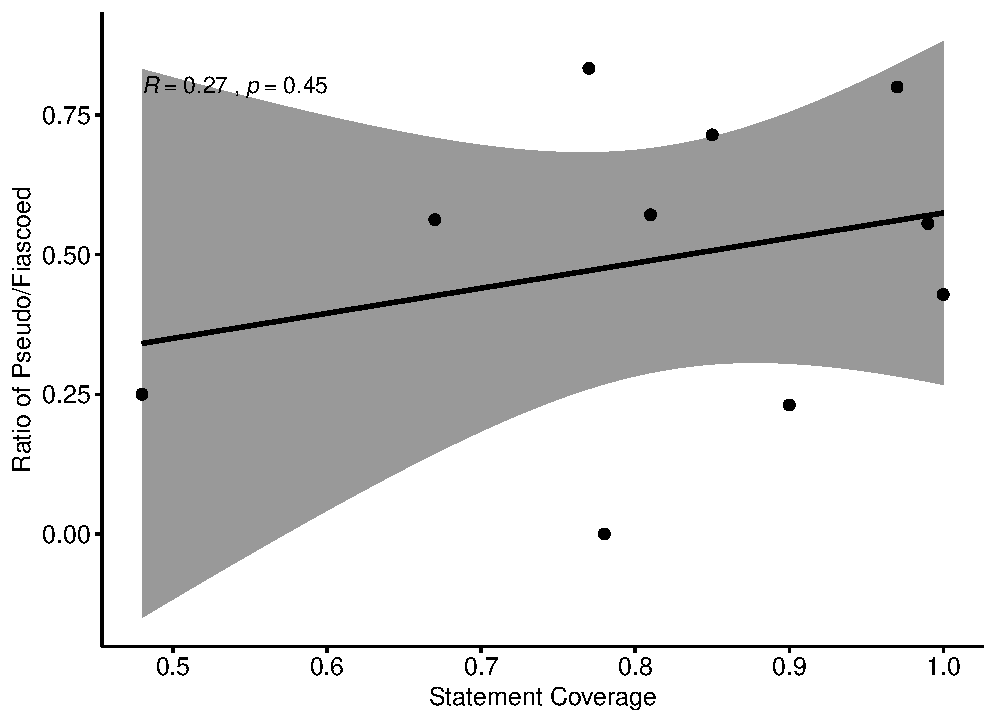
\includegraphics[scale = .5]{images/stateCovPlot}
  \caption{Correlation between the Statement Coverage and a ratio of ``fiascoed'' methods and the number of pseudo-tested methods.}~\label{stateCovReg}
\end{figure}


% * Full result and what it means
The overall result of the experimentation is that pseudo-tested methods are an issue that is affecting systems that are far along in their maturity and systems that are still implementing features. Systems that had lower percentages for their statement coverage were found to have less pseudo-tested methods in their systems. However, this could be explained by the amount of functions that were not being executed as this group could have tested functions in the future that are actually being pseudo-tested. It does follow that the systems that have more tests tend to have more pseudo-tested functions, but this is a product of the sheer number of tests.

The execution of Function-Fiasco resulted in the support for the findings of~\cite{niedermayr2016will}~\cite{vera2017comprehensive}. Both studies concluded with the existance of pseudo-tested methods in Java based systems. The results of this research also concludes that pseudo-tested methods exist in Python based systems. The combination of the findings allows for the inference that pseudo-tested methods can be found in many languages outside of Python and Java. The two languages are completely different when it comes to type safety. Java will force an exception if the type of a variable is overwritten, while Python will allow this computation to occur. There are many languages that are like Java and Python that may experience those same testing vulnerabilities.

It was also discovered that \texttt{Strings} and \texttt{Booleans} are more likely to create a scenario for a pseudo-tested method. For each primitive type of return for functions, the number of the functions present was put into a ratio with the number of functions with that type that were pseudo-tested. Table \ref{retTable} shows a breakdown of the return types that resulted in the most pseudo-tested methods. While some types were used significantly more than others, the ratio of the types explains this reasoning. Both \texttt{Strings} and \texttt{Booleans} are found to produce a pseudo-tested method over half of the time. The number of \texttt{Booleans} that were found to be pseudo-tested may be skewed due to the large number of intentional pseudo-testing that GatorGrader was employing.

% latex table generated in R 3.5.3 by xtable 1.8-3 package
% Tue Apr  2 04:08:23 2019
\begin{table}[H]
\centering
\begin{tabular}{rlrrl}
  \hline
 & Type & Used & Found & ratio \\
  \hline
1 & Strings &  69 &  33 & 47.8\% \\
  2 & Booleans &  49 &  35 & 73.5\% \\
  3 & Ints &  18 &   4 & 22.2\% \\
  4 & Floats &   1 &   0 & 0\% \\
   \hline
\end{tabular}
\caption{Breakdown of the number of pseudo-tested method per type.}~\label{retTable}
\end{table}


%   * In general the systems that have more methods and are further into the maturity of their systems generally contain less pseudo-tested methods
%   * This may be an incorrect statement as the number of functions that can be fiascoified is increased.



% ###############################################################################################################
%                                     End of Experimentation
% ###############################################################################################################
% TODO
% MAYBE ADD THIS SECTION
% * Examples of pseudo-tested methods

% \subsection{Examples of pseudo-Tested Methods}
%
% Since many pseudo-tested methods were found in each system, it is important to mention the different reasons as to why they are being pseudo-tested.

% ###############################################################################################################
%                                     End of Examples
% ###############################################################################################################
%

\section{Threats to Validity}
The threats to the validity of the research are separated into three sections which are based on how the threat would affect the validity of the research. The sections are internal validity, the function coverage, and the confirmability of pseudo-tested methods.

\subsection{Internal Validity}
% TODO determine if the verbage should be researchers or researcher
% * All of the tools that were created to detect the presence of pseudo-tested methods were created by the researcher.
% * Leverages the use of the other made systems, means that if one of them is wrong, the whole result could be

The largest internal threat to validity is the fact that all of the tools that are used in the detection of pseudo-tested methods, with the exception of libraries that are standard to the Python programming language and Pytest, were made by the researcher. This includes the module reloading plugin pytestReload, the impact analysis assistance pytestFinder, and Function-Fiasco which is making the final determination as to what functions are being pseudo-tested. One major effect that this environment can have is the idea that some functions are being left out. Function-Fiasco relies on the passing of test cases to determine if the function is pseudo-tested. There are many tests that pass in the normal setup of the system, but when run from afar with a different configuration the extra step will force them to fail. Which means that the function is not being fully tested for its pseudo-testedness. This could mean that the numbers that were presented in Section \ref{sec:Experiments} could be even higher. Since the research was very intensly tested on the system GatorGrader~\cite{Gat}, which is a system of moderate size with high coverage, it is believed that the number of pseudo-tested methods being present in this system that are untested could be high. This is because Function-Fiasco is very early on in its development maturity. Function-Fiasco is only able to handle a small amount of possibilities when it comes to type returns and object oriented design. This means that many functions in systems, both large and small, are being ignored and not ``fiascoed''. They are still checked to see if they are tested, but they are not analyzed for pseudo-testedness. This means that any of the functions of that are ignored are possibly pseudo-tested.

% ###############################################################################################################
%                                     End of Internal Creation
% ###############################################################################################################

\subsection{Function Coverage}

% * Function coverage does not explain the coverage of a system in a great detail.
%   * Methods that are not tested may not contain a large number of statements, while others do
%   * Blanking

The function coverage that is produced is helpful to understand how many of the system's functions are being tested. This type of insight provides an overhead view of the general behavior of the system. There is an issue with function coverage though, and it is that it is general. One of them most common types of coverage used in industry is statement coverage. Statement coverage is a marker to determine how many of the individual statements are being tested throughout the execution of the system's test suite. This is why the statement coverage of a system could be drastically different from the function coverage. For example, assume there was a function that was not being tested that contains few lines and that there is a function that is being tested that contains a large amount of lines. After the statement and function coverage had been calculated, they would be very different. The function coverage would be affected in a more significant way assuming that there is a small amount of functions in the system. The statement coverage would be affected in a minor way that could be represented with a subtraction of a low number of percentage points. While this would explain the discrepancy in the two types of coverage, it is worth noting because of the adjusted function coverage. To combat this type of threat, the statement coverage is presented to the user as well so that if the function coverage is lower than expected, the user has another metric to base the changes off of.

Another threat to validity involving the function coverage is a term that was created during the implementation phase of the system. This term will be referred to as ``blanking''.  Function-Fiasco relies on the test suite of the system running tests that cause the decorator that is applied to be activated so that the return type of the function under scrutiny is relayed back to Function-Fiasco. If no tests are executed, this return type is ignored and the function is referred to as untested. There is a case where tests are executed for a function, but based on the configuration of the system or tests that were already resulting in a failed case, the test would fail or error before the decorator has the ability to be activated. This would result in the type of the return in the function being relayed to Function-Fiasco as a blank line. Since there were tests executed, the function is still referred to as tested, but it was not ``fiascoed.'' Therefore, this case is referred to as ``blanked''. The blank line is persistant because of the initialization of the variable that stores the return type. It is initialized as an empty string and is unchanged after the execution. This case affects the function coverage because it is still referred to as tested, and forces to the function coverage to remain high. However, the function is not ``fiascoed'' so it is not considered to be checked for its pseudo-testedness. This could result in the function coverage not being accurately corrected after Function-Fiasco finishes its execution.

% ###############################################################################################################
%                                     End of Function Coverage
% ###############################################################################################################

\subsection{Confirmability}

% * Hard to confirm if the output of a large system is correct.
%   * Hand check for pseudo-tested methods to confirm accuracy
%   * Large systems with many require too much time to verify every circumstance
% * Configuration issues may lead to inaccuracy
%   * Based on configuration there may be tests that cannot be run
%   * There is a chance that the fuzzing returned a state that could still be accurate enough to create a passing test case.

Another large threat to the the validity of the research is that the accuracy is very difficult to detect. Since pseudo-tested methods can already be hard to detect by the developer, it is hard to confirm that the system that detects them is working accurately. One major reason is the potential functionality swallowing. It is possible to see that a function is passing a test case when it shouldn't if the test has an assertion that can never fail, but it is difficult to find a function whose functionality is being ignored throughout the systems execution. To accomplish this, a developer needs to follow the execution trail that the function can leave. This means following every function call that the function receives, recognizing what the output should be, and determining if this output truly has an effect on the system as a whole. This can be especially difficult based on the size and the complexity of the system. A function could be used by a numerous amount of other functions. This could make it very difficult to trace the execution trail of a function. It could take too much time and would make using Function-Fiasco redundant. Therefore Function-Fiasco is operating under the assumption that the execution is accurate in detecting pseudo-tested methods with a high degree of certainty. Function-Fiasco has been hand checked on the system GatorGrader~\cite{Gat}, which is a medium-sized system with 100\% coverage and thorough documentation. This means that Function-Fiasco has been checked by hand for a system that contains a plethora of different scenarios to experience.

Another issue that could make it hard to confirm the accuracy of the system is that of configuration issues. It is possible that the configuration of the system that is being tested produces tests that are not able to pass because the configuration from being executed from a directory is not the same as being executed from the root directory of the system. In many cases that are similar to this, the test will error before the function could blank, leaving the possibility of the coverage not being updated to a correct number because of remaining pseudo-tested methods in the system that were not executed. The other threat to the confirmability of Function-Fiasco is the use of fuzzing. Since fuzzing is providing the basis to what is being pseudo-tested or not, there is a chance that the randomized return could create a state that makes the test pass, instead of creating a state where the test should fail but passes anyway. An example of this would be a function that is meant to produce a number within a range, such as an angle for a triangle. In this case any angle that is still valid for a triangle would be accepted and the return produced could satisfy this. To combat this the range that the fuzzing would produce for a number is between 1 and 100, strings are made into an arrangement of random characters, and booleans were returned with an arbitrary number.

% ###############################################################################################################
%                                     End of Confirmability
% ###############################################################################################################

\begin{figure}[t!]
\begin{lstlisting}[language = Python, frame = single, caption = Contents of fake.py, label = fakepy]
def decorate(func):
    def dec(*args, **kwargs):
        return func(*args, **kwargs)
    return dec

def length():
    size()
    return 6

@decorate
def search():
    return "asdfjkl;"

def addition():
    calculate()
    return 5.01019292

def calculate():
    return True

def tester():
    a = classCheck2()
    a.hello2()
    return

def checkOutput():
    return []

class classCheck():
    def hello(self):
        print("hello")

class classCheck2():
    def hello2(self):
        return 10
\end{lstlisting}
\end{figure}
